\subsection{Caso d'uso UC4: Logout}
	\label{UC4}
	\begin{figure}[h]
		\centering
			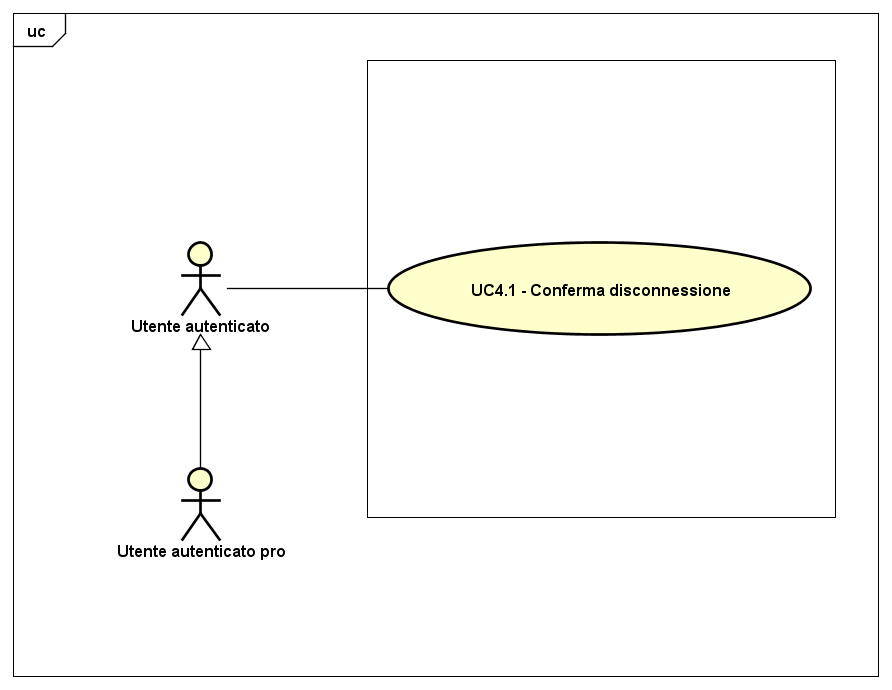
\includegraphics[scale=0.5,keepaspectratio]{UML/UC4.png}
		\caption{UC4: Logout}
	\end{figure}
	\FloatBarrier
	\begin{itemize}
		\item
			\textbf{Attori}: utente autenticato, utente autenticato pro;
		\item		
			\textbf{Descrizione}: l'attore termina la sua sessione, uscendo dalla sua area riservata;
		\item
			\textbf{Precondizione}: l'attore è autenticato presso il sistema;
		\item
			\textbf{Postcondizione}: l'attore non è autenticato presso il sistema;
		\item
			\textbf{Scenario principale}:
	       		\begin{itemize}
					\item
					L'attore riceve la conferma della disconnessione (UC4.1).
	 			\end{itemize}
	\end{itemize}

\subsubsection{Caso d'uso UC4.1: Conferma disconnessione}
	\begin{itemize}
		\item
			\textbf{Attori}: utente autenticato, utente autenticato pro;
		\item
			\textbf{Descrizione}: l'attore, una volta selezionato l'opzione logout, attende la conferma della disconnessione da parte del sistema;
 		\item
			\textbf{Precondizione}: l'attore ha selezionato l'opzione logout;
		\item
			\textbf{Postcondizione}: Il sistema conferma all'attore l'uscita dalla sua area riservata;
		\item
			\textbf{Scenario principale}: l'attore riceve conferma del logout.
	\end{itemize}		
	